\def\ty{\tilde{y}}
\def\sh{\mathrm{sh}}
\def\ch{\mathrm{ch}}

\begin{remark}
  Дана теорема є незручною для розв'язання задач. Для того, щоб встановити більш зручну теорему, потрібна \textit{Лема Лагранжа}.
\end{remark}

\begin{lema}
  Якщо $f\in C[a,b]$ і $ \int\limits_{a}^{ b}{f(x)h(x) \mathrm{d}x} =0\ :\
  \forall h \in C^1[a, b] : h(a) = h(b) = 0
  $,
  $$
  \textbf{Тоді:} \qquad f(x) = 0 \ \ \forall x \in [a,b]
  $$
\end{lema}
\begin{proof}
 Припустимо від супротивного, що $\exists x_0 \in [a,b] : f(x_0) \neq 0.$ Візьмемо $f(x_0)>0$. Оскільки $f \in C[a,b]$, то існує окіл цієї точки: $O_{\varepsilon } (x_0) = (x_0 - \varepsilon , x_0 + \varepsilon )$ такий, що: $\forall x \in O_{\varepsilon }$. Візьмемо:
 $$
 h(x) = \begin{cases}
  (x-(x_0 -\varepsilon ))^2(x-(x_0 +\varepsilon ))^2, & x \in O_{\varepsilon};\\
  0,  & x \notin O_{\varepsilon}.
 \end{cases} \quad \begin{gathered}
  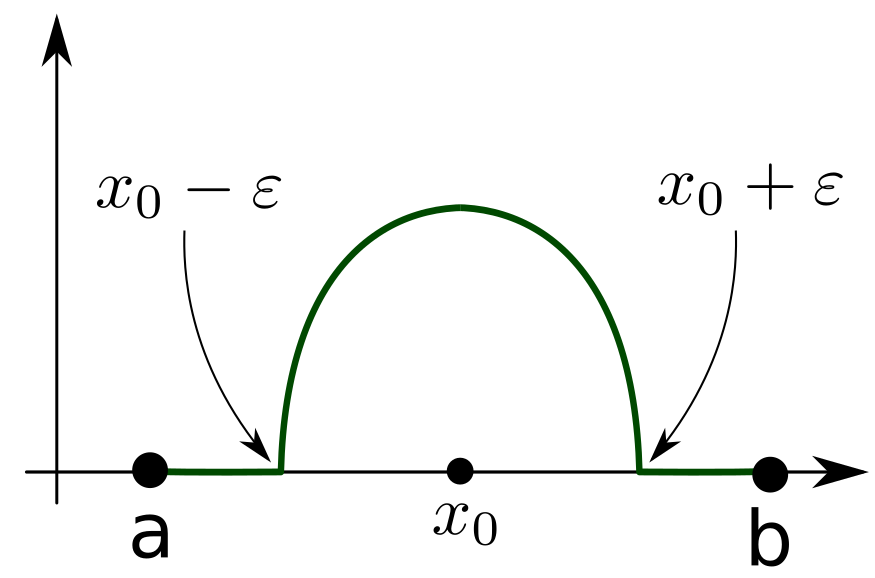
\includegraphics[scale=0.17]{assets/lectures_recent-91d0043b.png}
 \end{gathered}
 $$
 Тоді $h(x) \in C^1 [a,b], h(a) = h(b) = 0$. При цьому:
 $$
 0 =  \int\limits_{a}^{b}{f(x)h(x) \mathrm{d}x} =  \int\limits_{x_0 + \varepsilon}^{ x_0 - \varepsilon}{\underbrace{f(x) h(x)}_{ > 0 \text{ за прип.}}\mathrm{d} x } > 0
 $$
 Отримали протирічча $0 > 0$.
\end{proof}
\begin{boxteo}
 Нехай $F(x,y,p)  \in C^2([a,b] \times \mathbb{R}^2)$ - задана функція.\\ Нехай допустима функція $\tilde{y} \in C^2[a,b]$ є розв'язком найпростішої з.в.ч.\\
 Тоді $\tilde{y}(x)$ задовільняє рівняння Ейлера на $[a,b]$:
 $$
 \frac{\d F}{\d y} - \frac{\mathrm{d} }{\mathrm{d} x} \frac{\d F}{\d y'} =0
 $$
\end{boxteo}
\newpage
\begin{proof}
Нехай  $\tilde{y} \in C^2[a,b]$ є розв'язком найпростішої з.в.ч. Тоді:
$$
\delta J(\tilde{y}, h) = 0 \qquad \forall h \in C^1 [a,b] : h(a) = h(b) = 0
$$
$$
0 = \delta J(\tilde{y}, h) = \frac{\mathrm{d}}{\mathrm{d}\alpha} J(\tilde{y} + \alpha h) \vline_{\alpha=0} =
  \int\limits_{a}^{b}{ \frac{\d F}{\d y} (x, \tilde{y}, \tilde{y}') \cdot h(x) + \frac{\d F}{\d y'} (x, \tilde{y}, \tilde{y}') \cdot h'(x)
 } =$$$$= \left|
\begin{gathered}
 u =   \frac{\d F}{\d y'} (x, \tilde{y}, \tilde{y}')\\
 du = \frac{\mathrm{d} }{\mathrm{d} x} \left(  \frac{\d F}{\d y'} (x, \tilde{y}, \tilde{y}') \right)
\end{gathered} \ \
\begin{gathered}
 dv = h' (x ) \mathrm{d}x \\
 v = h(x)
\end{gathered}
  \right| =   \int\limits_{a}^{b}{ \frac{\d F}{\d y} (x, \tilde{y}, \tilde{y}') \cdot h(x) \mathrm{d} x} +
$$
$$
+ \underbrace{ \left. \frac{\d F}{\d y'} (x, \tilde{y}, \tilde{y}') \cdot h(x) \right|_{a}^b}_{ = 0 \ \Leftarrow \ h(b) = h(a) = 0}  -  \int\limits_{a}^{ b}{\frac{\mathrm{d} }{\mathrm{d} x} \left(  \frac{\d F}{\d y'} (x, \tilde{y}, \tilde{y}') \right) \cdot h(x) \mathrm{d} x} =
$$
$$
 =  \int\limits_{a}^{b}{ \left[
 \frac{\d F}{\d y} (x, \tilde{y}, \tilde{y}')
  - \frac{\mathrm{d} }{\mathrm{d} x} \left(  \frac{\d F}{\d y'} (x, \tilde{y}, \tilde{y}') \right)
  \right]\cdot h(x) \mathrm{d} x} = 0
$$
$$
\forall h \in C^1[a,b] : h(a) = h(b) = 0 \xRightarrow{\text{лема Лагранжа}} \text{ р-ня Ейлера.}
$$
\end{proof}
\begin{defo}
  Розв'язки рівняння Екйлера називаються \textbf{екстремалями} функціоналу $J(y)$. Екстремалі, які є допустимими функціями, називаютсья \textit{допустимими екстремалями}. Саме серед допустимих екстремалей слід шукати розв'язок НЗВЧ.
\end{defo}
\begin{remark}
  Умови $\tilde{y} \in C^2[a,b] , F\in C^2 \left( [a,b] \times \mathbb{R}^2 \right)$ накладені з метою спростити доведення (щоб ''узаконити'' інтегрування частинами). Насправді, твердження теореми буде вірним і для неперервно-диференційованих функцій.
\end{remark}
\begin{example}
 $$
 \begin{dcases}
   \int\limits_{0}^{ 1}{(y'(x))^2 \mathrm{d} x} \to \mathrm{extr};\\
   y(0) = 0 \qquad y(1) = 1.
 \end{dcases}
 $$
 \begin{enumerate}
   \item Складаємо і розв'язуємо рівняння Ейлера:
   $$
   \frac{\d F}{\d y} - \frac{\mathrm{d} }{ \mathrm{d} x} \frac{\d F}{\d y'} = 0
   $$
   $$
   F(x,y,y') = (y')^2 \qquad \frac{\d F}{\d y} = 0 \qquad \frac{\d F}{\d y'} = 2y'
   $$
   $$
   \frac{\mathrm{d}}{\mathrm{d} x} \frac{\d F}{ \d y'} = \frac{\mathrm{d}}{\mathrm{d} x} (2 y') = 2 y''  \ \Longrightarrow \
   0 - 2y'' = 0 \ \Longrightarrow \  \fbox{$y'' = 0$}
   $$
   Отримали рівняння Ейлера. Двічі інтегруємо:
   $$
   y = C_1 x + C_2 \text{ --- сімейство екстремалей.}
   $$
   \item Знаходимо допустимі екстремалі.
   $$
   y(0) = 0 \ \Rightarrow \  0 = C_1 \cdot 0 + C_2 \ \Rightarrow \  C_2 = 0
   $$
   $$
   y(1) = 1 \ \Rightarrow \  1 = C_1 \cdot 1 \ \Rightarrow \  C_1 = 1
   $$
   $$
   \tilde{y}(x) = x \text{ --- допустима екстремаль.}
   $$
   \item Перевіряємо, чи досягаєтся в $\tilde{y} (x)\  \mathrm{extr}$ функціоналу $J(y)$:\\
   $
   \forall h \in C^1 [0,1] : h(0) = h(1) = 0
   $ розглядаємо $J(\tilde{y} + h) - J(\tilde{y})$.\\
 \end{enumerate}

 \newpage

 \begin{itemize}
   \item    Якщо $J(\tilde{y}+ h) - J(\tilde{y})  \geq 0 \ \ \forall h \in C^1 [0,1] : h(0) = h(1) = 0$  принаймі з деякого околу $||h||_{C^1 [0,1]} < \delta$, то $\tilde{y} (x) $ забезпечує слабкий локальний мінімум функціоналу.
   \item Якщо $J(\tilde{y}+ h) - J(\tilde{y})  \geq 0 \ \ \forall h \in C^1 [0,1] : h(0) = h(1) = 0$, то $\tilde{y} (x) $ забезпечує слабкий глобальний мінімум функціоналу.
   \item Якщо нерівність виконується з протилежним знаком ($ \leq 0$), то досягається максимум (локальний або глобальний).
   \item Якщо різниця функціоналів знакозмінна, то extr не досягається.
 \end{itemize}
 Маємо:
 $$
 J(\tilde{y} + h) - J(\tilde{y}) =  \int\limits_{0}^{1}{ (\tilde{y}' + h')^2 \mathrm{d}x} -  \int\limits_{0}^{ 1}{ (\ty')^2 \mathrm{d} x} =
 $$
 $$
 =  \int\limits_{0}^{ 1}{ (\ty')^2  + 2 \ty'h' + h'^2  -  (\ty')^2 \mathrm{d}x} \oeq
 $$
 $$
 \left(  \int\limits_{0}^{1}{ \ty' h'} =  \left|  \begin{gathered}
  \ty' = u\\
  \ty'' = \mathrm{d}u
 \end{gathered}\ \ \begin{gathered}
  h' = v' \\
  h = v
 \end{gathered} \right| = \ty' h\bigg|_0^1 -  \int\limits_{0}^{1}{ \ty'' h \mathrm{d}x} = 0 \right)
 $$
 $$
 \oeq  \int\limits_{0}^{1}{ (h')^2 \mathrm{d}x} \geq  \quad \forall h \in C^1[0,1] : h(0) = h(1) = 0 \Longrightarrow \fbox{сл. глобальний мінімум.}
 $$
\end{example}
\newpage
\begin{example}
 $$
 \begin{dcases}
  J(y) =  \int\limits_{0}^{1}{ (y + y')^2 \mathrm{d} x} \to \mathrm{extr}\\
  y(0) = 1 \qquad y(1) = 0
 \end{dcases}
 $$
\end{example}
\begin{enumerate}
  \item Складаємо і розв'язуємо рівняння Ейлера:
  $$
  F = (y + y')^2 \qquad \frac{\d F}{\d y} = 2(y + y') \qquad \frac{\d F}{\d y'} = 2(y + y')
  $$
  $$
  \frac{\d F}{\d y} - \frac{\mathrm{d} }{\mathrm{d}x } \frac{\d F}{\d y'} = 0
  $$
  $$
  y + y' - \frac{\mathrm{d} }{\mathrm{d} x} (y + y') = 0
  $$
  $$
  y + y' - y' - y'' = 0 \ \ \Longrightarrow \ \  y'' - y = 0  \textit{ --- рівняння Ейлера.}
  $$
  Отримали ЛОР 2-го порядку. Складемо характеристичне рівняння:
  $$
  \lambda^2 - 1 = 0 \ \Longrightarrow \  \lambda= \pm 1 \ \Longrightarrow \  y(x) = C_1 + e^x + C_2 e^{-x} \text{-- сімейство екстремалей.}
  $$
  \item Знаходимо допустові екстремалі:
  $$
  \begin{array}{l c c c}
    y(0) = 1 : & 1 = C_1 e^0 + C_2 e^0  & \Longrightarrow & C_1 + C_2 = 1\\
    y(1) = 0 : & 0 = C_1 e^{1} + C_2 e^{-1}  & \Longrightarrow & C_1 + C_2e^{-2} = 0\\
  \end{array} \Rightarrow
  \begin{cases}
    C_1 + C_2 = 1\\
    C_1 + C_2e^{-2} = 0
  \end{cases}
  $$
  $$
  C_2 (e - e^{-1}) = e  \quad  \Longrightarrow \quad C_2 = \frac{e}{e - e^{-1}}  \quad \Longrightarrow \quad C_1 = - \frac{1}{e ( e - e ^{-1})}
  $$
  $$
  \ty (x) =  - \frac{1}{e ( e - e ^{-1})}  e^{x} + \frac{e}{e - e^{-1}} e^{-x} = \frac{1}{e - e^{-1}}  \left(  - e^{x-1} + e^{-x +1} \right) = - \frac{\sh(x-1)}{\sh(1)}
  $$
  Отримали $- \frac{\sh(x-1)}{\sh(1)}$ --- допустима екстремаль.
  \item Перевірка. Перевіряємо, чи забезпечує $\ty (x) $ екстремум задачі.\\
  $
  \forall h \in C ^1 [0,1] : h(0) = h(1) = 0:
  $
  $$
  J(\ty  + h ) - J(\ty) =  \int\limits_{0}^{1}{ ((\ty + h) + (\ty' + h'))^2 \mathrm{d}x} -  \int\limits_{0}^{1}{
  (\ty + \ty')^2 \mathrm{d}x
  } =
  $$
  $$
  =  \int\limits_{0}^{1}{ (\ty + h)^2 + 2 (\ty + h) (\ty' + h') + (\ty' + h')^2 \mathrm{d} x} -  \int\limits_{0}^{1}{ \ty^2 + 2 \ty\ty' + (\ty')^2 \mathrm{d}x} =
  $$
  $$
  = \left|  \textit{розкриваючи дужки} \right| =  \int\limits_{0}^{1}{ h^2 + (h')^2 + 2 (\ty + \ty') h + 2(\ty + \ty')h' \mathrm{d} x } \oeq
  $$
  $$
  \left( \begin{gathered}
   \text{ Візьмемо частинами:} \\
 \int\limits_{0}^{1}{ (\ty + \ty')h' \mathrm{d}x} = \left|  \begin{gathered}
  (\ty + \ty') = u \\
  (\ty' + \ty'' ) = \mathrm{d} u
 \end{gathered} \ \begin{gathered}
  h' = v' \\
  h = v
 \end{gathered} \right| = \ \\
 = \underbrace{(\ty + \ty')h \bigg|_{0}^{1}}_{ = 0 \ \Leftarrow \ h(0)=h(1)=0 } -  \int\limits_{0}^{1}{(\ty' + \ty'' )h \mathrm{d}x}
  \end{gathered} \right)
  $$
  $$
  \oeq  \int\limits_{0}^{1}{h^2 + (h')^2 + \underbrace{2 (\ty + \ty' - \ty' - \ty'')}_{=0 \ \Leftarrow \ \ty = \ty'' (\text{з р-ня Ейлера})h} \mathrm{d}x} =
  $$
  $$
  =  \int\limits_{0}^{1}{ (h^2 + (h')^2)\mathrm{d}x} \geq 0 \qquad
   \forall h \in C^1[a,b] : h(0) = h(1) = 0
  $$

  Отримали: \fbox{$\ty(x) = -\frac{\sh(x-1)}{\sh(1)} $ --- слабкий глобальний мінімум функціоналу.}
\end{enumerate}
\subsection{Задача про брахісторону}
Знайти криву, по якій матеріальна точка скотиться найшвидше, нехтуюч тертям та опорою середовища.
Нехай т. $A$ - т. початку координат. т. $B (x_1, y_1)$.
$$
\begin{gathered}
 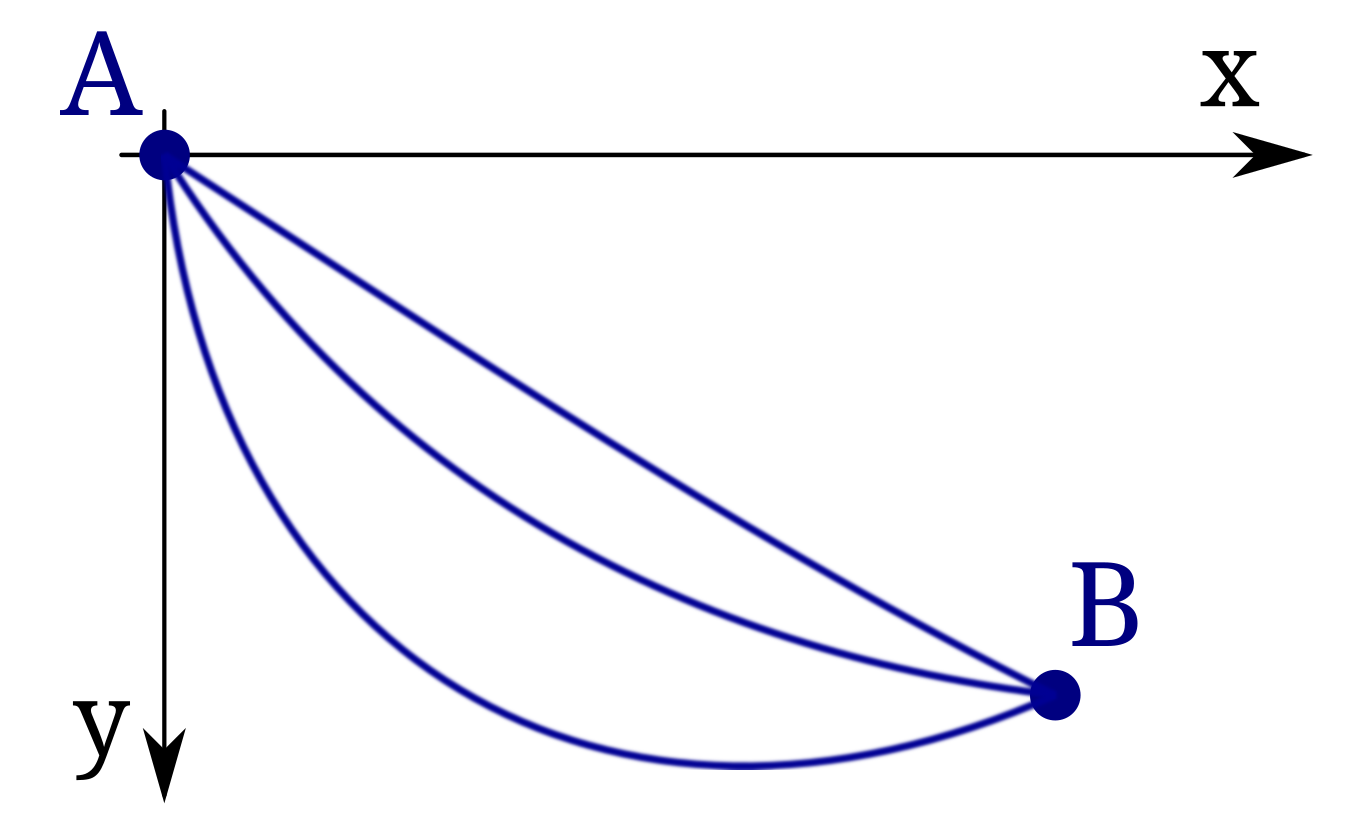
\includegraphics[scale=0.2]{assets/lectures_part_3-91d0349d.png}
\end{gathered}
\qquad \quad
\begin{gathered}
U(x) = \frac{\mathrm{d} s}{ \mathrm{d} t} \ \Longrightarrow \ \mathrm{d}t = \frac{\mathrm{d} s}{U(x)}\\
\mathrm{d} s = \sqrt{1 + (y')^2} \mathrm{d} x\\
\text{Закон збереження енергії:}\\
\frac{mv^2}{2} = mgy \ \Longrightarrow \  v = \sqrt{2gy} \\
\mathrm{d}t = \dfrac{\sqrt{1 + (y')^2} \mathrm{d} x}{\sqrt{2gy}}
\end{gathered}
$$
Отримали математичну постановку задачі:
$$
\begin{dcases}
 t = \frac{1}{2g}  \int\limits_{0}^{x_1}{ \sqrt{ \frac{1+ (y')^2}{y} } \mathrm{d} x} \to \mathrm{extr}\\
 y(0) = 0 \qquad \quad y(x_1)  = y_1
\end{dcases}
$$
Класичне рівняння Ейлера надто складне для даної задачі.
\begin{lema}
  Якщо $F(x,y,y') = F(y, y')$ (не залежить від $x$), то рівняння Ейлера набуває вигляду:
  $$
  \frac{\mathrm{d}}{\mathrm{d} x} \left( F - y' \frac{\d F}{ \d y'}  \right) = 0
  $$
\end{lema}
